\documentclass[a4paper, 12pt]{article}

\makeatletter
\newenvironment{sqcases}{%
  \matrix@check\sqcases\env@sqcases
}{%
  \endarray\right.%
}
\def\env@sqcases{%
  \let\@ifnextchar\new@ifnextchar
  \left\lbrack
  \def\arraystretch{1.2}%
  \array{@{}l@{\quad}l@{}}%
}
\makeatother

\usepackage[top=2cm, bottom=2cm, left=2cm, right=2cm]{geometry}
%\renewcommand{\baselinestretch}{1.65}
%\newcommand{\jj}{\righthyphenmin=20 \justifying}
\usepackage{ragged2e}
\justifying
\usepackage{booktabs}
\usepackage[russian]{babel}
\usepackage{amssymb}
\usepackage{enumerate}
\usepackage{units}
\long\def\comment{}

\newtheorem{theorem}{Theorem}
\newtheorem{lemma}{Lemma}

\usepackage{tikz}
\usepackage{tikz-3dplot}

\usepackage{caption}
\usepackage{subcaption}
\usepackage{graphicx}

\graphicspath{{./pictures/}}
\DeclareGraphicsExtensions{.pdf,.png,.jpg,.svg}

\usepackage{pdfpages}
\usepackage{amsmath}
\usepackage{textcomp}
\usepackage{gensymb}
\usepackage{physics}

\newcommand*\diff{\mathop{}\!\mathrm{d}}
\newcommand{\slfrac}[2]{\left.#1/#2\right.}
\newcommand{\Int}[4]{\displaystyle \int_{#1}^{#2} #3 \diff #4}
\newcommand{\Intu}[3]{\displaystyle \int_{#1}^{#2} #3}

\addto\captionsrussian{\renewcommand{\figurename}{Fig.}}
\addto\captionsrussian{\renewcommand{\refname}{References}}
\renewcommand{\figurename}{Fig.}
\renewcommand{\refname}{References}

\begin{document}
	%-------------------------------------------------TITLE----------------------------------------------------------
	\begin{center}
		\large
		\textbf{National Research University}			
		\\
		\textbf{Higher School of Economics}									\\[3 cm]
		\textbf{Moscow Institute of Electronics and Mathematics}			\\[2 cm]
									
	\end{center}
	
	\begin{center}
		\large
		\textbf{Department of Applied Mathematics}		\\[3 cm]
	\end{center}
	
	
	
	\begin{center}
		\large
		\textbf{Calculation of Electron Spectrum in Spherically Symmetric Potentials}		\\[6 cm]
		
	\end{center}
	
	\begin{flushright}
		\large
		\textbf{Orlova Elena Gennagyevna}				\\
		\textbf{Scientific Supervisor:}			\\
		\textbf{Ikhsanov Renat Shamil’evich}		\\
	\end{flushright}
	
	\vfill
	\begin{center}
		\large
		\textbf{Moscow 2017}
	\end{center}
	\pagebreak
	
	
	
    %-------------------------------------------------------------1-----------------------------------------------------------
		
\section{Introduction}

An important problem in quantum mechanics is a benaviour of a particle in a spherically symmetric potential, which depends only on the distance between the particle and a defined center point. An electron in the potential derived from Coulomb's law is well-known example. The problem can be used to describe a hydrogen-like atom. 


The spectrum of particle consists of all possible values of energy. The study of particle spectra allows us to see the global picture of particle behavior. 


We are interested in finding a spectrum of electron in spherically symmetric potentials, such as: infinite and finite spherical potential well, quadratic potential, hydrogen-like atom; Woods-Saxon, Hulthen, Morse, Yukawa potentials and deuterium potential.


\section{Theoretical part}
\subsection{Differential operators in spherical coordinates}\label{dif_op_3d}


Suppose we have standard three dimension axes . A spherical coordinate system is a coordinate system where the position of a point is specified by three quantities: the radial distance $r$ of that point from the origin, its polar angle $\theta$ measured between polar axis (positive $z$-axis) and the line from the origin to the point, and the azimuth angle $\phi$ between the positive $x$-axis  and the line's from the origin to the point orthogonal projection on a reference plane $Oxy$.


\tdplotsetmaincoords{60}{110}
%
\pgfmathsetmacro{\rvec}{.8}
\pgfmathsetmacro{\thetavec}{30}
\pgfmathsetmacro{\phivec}{60}
%
\begin{figure}[h!]
\begin{center}
\begin{tikzpicture}[scale=5,tdplot_main_coords]
    \coordinate (O) at (0,0,0);
    \draw[thick,->] (0,0,0) -- (1,0,0) node[anchor=north east]{$x$};
    \draw[thick,->] (0,0,0) -- (0,1,0) node[anchor=north west]{$y$};
\draw[thick,->] (0,0,0) -- (0,0,1) node[anchor=south]{$z$};
    \tdplotsetcoord{P}{\rvec}{\thetavec}{\phivec}
    \draw[-stealth,color=red] (O) -- (P) node[above right] {$P$};
    \draw[dashed, color=red] (O) -- (Pxy);
    \draw[dashed, color=red] (P) -- (Pxy);
    \tdplotdrawarc{(O)}{0.2}{0}{\phivec}{anchor=north}{$\phi$}
    \tdplotsetthetaplanecoords{\phivec}
    \tdplotdrawarc[tdplot_rotated_coords]{(0,0,0)}{0.5}{0}%
        {\thetavec}{anchor=south west}{$\theta$}
\end{tikzpicture}
\end{center}
\caption{Spherical coordinates}
\end{figure}
Cartesian coordinates to Spherical coordinates:
\begin{equation} \label{sph_coord}
\begin{cases}
	{x}= {r} \sin{\theta}\cos{\phi} \\
	{y} = {r} \sin{\theta}\sin{\phi} \\
	{z} = {r}\cos{\theta}
\end{cases}
\end{equation}


Laplacian is a differential operator given by the divergence of the gradient of a function on Euclidean space. Laplace operator in Cartesian coordinates:
 	$$\nabla^2= \frac{\partial^2}{\partial x^2}  + \frac{\partial^2}{\partial y^2} + \frac{\partial^2}{\partial z^2}$$
So, using \eqref{sph_coord} we can find Laplasian in spherical coordinates:
\begin{equation}\label{sph_lap}
	\nabla^2 = \frac{1}{r^2} \frac{\partial}{\partial r}({r^2}\frac{\partial f}{\partial r})+\frac{1}{r^2\sin{\theta}}\frac{\partial}{\partial \theta}(\sin{\theta}\frac{\partial f}{\partial \theta})+\frac{1}{r^2\sin^2{\theta}}(\frac{\partial^2 f}{\partial \phi^2})
\end{equation}
Spherical coordinates are specially convenient in case when particle potential depends only on distance from some point.


\subsection{Some  necessary special functions}
For working with Laplasian in spherical coordinates several special functions often appear. We will describe them in two following paragraphs.
\subsubsection{Spherical functions}
Spherical harmonics are the angular part of the family of orthogonal solutions of the Laplace equation written in spherical coordinates \eqref{sph_lap}:
$$\nabla^2 {f} = \frac{1}{r^2} \frac{\partial}{\partial r}({r^2}\frac{\partial f}{\partial r})+\frac{1}{r^2\sin{\theta}}\frac{\partial}{\partial \theta}(\sin{\theta}\frac{\partial f}{\partial \theta})+\frac{1}{r^2\sin^2{\theta}}(\frac{\partial^2 f}{\partial \phi^2}) = 0$$
Suppose we can find solutions in the form $$f({r}, \theta, \phi) = R(r)Y(\theta, \phi)$$
Separation of variables gives two differential equations:
$$\frac{1}{R}\frac{\partial}{\partial r}(r^2 \frac {dR}{dr}) = \lambda$$
\begin{equation}\label{eq2}
	\frac{1}{Y}\frac{1}{\sin{\theta}}\frac{\partial}{\partial \theta}(\sin{\theta}\frac{\partial Y}{\partial \theta})+\frac{1}{Y}\frac{1}{\sin^2{\theta}}\frac{\partial^2 Y}{\partial \phi^2} = -\lambda
\end{equation}


The solution of \eqref{eq2} is represented in following form, called spherical garmonics of degree $l$ and order $m$:
\begin{equation}\label{sph_garm}
	Y_l^m(\theta, \phi)=\varepsilon \sqrt{\frac{(2l+1)}{4\pi}\frac{(l-|m|)!}{(l+|m|)!}}e^{im\phi}P_l^m(\cos{\theta}),
\end{equation}
 

where $\varepsilon = (-1)^m$ for $m\geq0$ and $\varepsilon=1$ for $m \leq 0$, $-l \leq m \leq l$ and $P_l^m $ is associated with Legendre Function, defined by:
	$$P_l^m(x)=(1-x^2)^{\frac{|m|}{2}}(\frac{d}{dx})^{|m|}P_l(x),$$
where $P_l(x) $ is Rodrigues formula:
	$$P_l(x) = \frac{1}{2^l l!}(\frac{d}{dx})^l (x^2-1)^l.$$


Notice, that $m$ and $l$ are integers. For any given $l$ there are $(2l+1)$ possible values for $m$: $l=0, 1...$, $m = -l, -l+1,..., -1, 0, 1, .., l-1, l.$


The general solution to Laplace's equation is linear combination of the spherical harmonic functions multiplied by the appropriate scale factor $r^l$:
	$$f(r, \theta. \phi) = \sum_{l=0} ^{\infty}\sum_{m=-l} ^{l}f_l^mr^l Y_l^m(\theta, \phi).$$
where the $f_l^m$ are constants.


\subsubsection{Bessel functions}
Bessel functions are canonical solutions $y(x)$ of following differential equation:
\begin{equation}\label{bess_eq}
x^2\frac{d^2 y}{dx^2}+x\frac{dy}{dx}+(x^2-\alpha^2)y = 0,
\end{equation}
where $\alpha$ is an arbitrary complex number, called the order of the Bessel function.

The most important cases are for $\alpha$ an integer or half-integer. Spherical Bessel functions with half-integer $\alpha$ are obtained when the Helmholtz equation is solved in spherical coordinates:
$$\nabla^2 A+k^2 A=0,$$
where $k$  is a wave number and $A$ is an amplitude.

When solving the Helmholtz equation in spherical coordinates by separation of variables, the radial equation has the form:
$$x^2\frac{d^2 y}{dx^2}+2x\frac{dy}{dx}+[x^2-n(n+1)]y = 0$$
The two linearly independent solutions to this equation are called the spherical Bessel functions $j_n$ and $y_n$:
\begin{equation}\label{bess_func1}
	j_n(x) = (-x)^n\bigg(\frac{1}{x} \frac{d}{dx}\bigg)^n \frac{\sin{x}}{x}
\end{equation}
\begin{equation}\label{bess_func2}
	n_n(x) = (-x)^n\bigg(\frac{1}{x} \frac{d}{dx}\bigg)^n \frac{\cos{x}}{x}
\end{equation}
\begin{figure}[h!]
\centering
\begin{subfigure}{.5\textwidth}
  \centering
  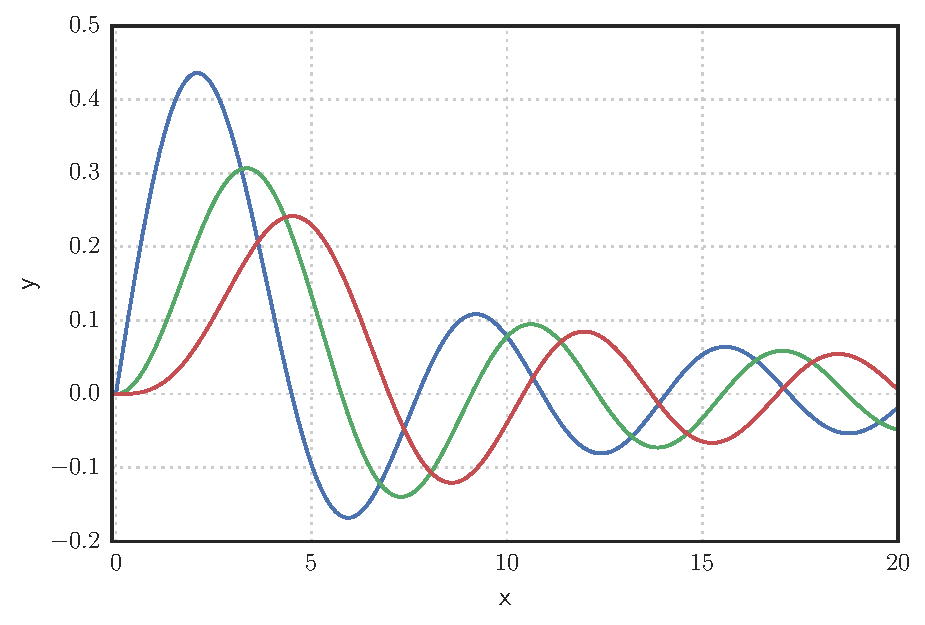
\includegraphics[width=1.0\linewidth]{bessel1.pdf}
  \caption{$j_n(x)$}
  \label{fig1:bessel1}
\end{subfigure}%
\begin{subfigure}{.5\textwidth}
  \centering
  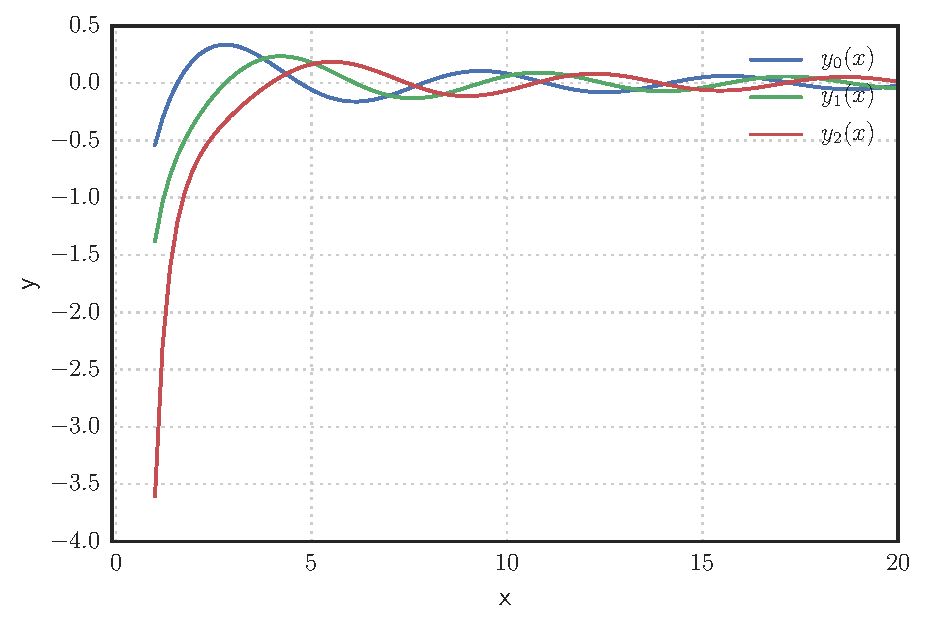
\includegraphics[width=1.0\linewidth]{bessel2.pdf}
  \caption{$y_n(x)$}
  \label{fig:bessel2}
\end{subfigure}
\caption{Spherical Bessel functions}
\label{fig:bessel}
\end{figure}


\subsection{Angular momentum}
The angular momentum $L$ of a material point relative to a reference point is determined by the cross product of particle's position vector $r$(relative to some origin) and its momentum vector $p$:
$$\mathbf{L = r \times  p},$$
which is to say,
%$$L_x=y p_z-z p_y, L_y=z p_x-x p_z, L_z=x p_y-y p_x$$%
$$\boldsymbol{L} = \begin{vmatrix} \boldsymbol{i} & \boldsymbol{j} & \boldsymbol{k} \\ 
x & y & z \\
p_x & p_y & p_z
\end{vmatrix}$$


This definition can be carried over to quantum mechanics, by reinterpreting $r$ as the quantum position operator   $\hat x=x$  and $p$ as the quantum momentum operator $\hat p=\frac{\hbar}{i}\nabla$:


$$\boldsymbol{L} = \frac{\hbar}{i}\begin{vmatrix} \boldsymbol{i} & \boldsymbol{j} & \boldsymbol{k} \\ 
x & y & z \\
\frac{\partial}{\partial x} & \frac{\partial}{\partial y} & \frac{\partial}{\partial z}
\end{vmatrix}$$

Writing this in coordinates, we obtain:

$$L_x = \frac{\hbar}{i}(y \frac{\partial}{\partial z}-z \frac{\partial}{\partial y}), ~L_y = \frac{\hbar}{i}(z \frac{\partial}{\partial x}-x \frac{\partial}{\partial z}), ~L_z = \frac{\hbar}{i}(x \frac{\partial}{\partial y}-y \frac{\partial}{\partial x})$$


In the next section we will consider the eigenvalues and eigenfunctions of these operators.

\subsubsection{Eigenvalues and eigenfunctions}
%Matrix multiplication is not, in general case, commutative; the difference between the two orderings is called commutator:
%$$[S, T] = ST-TS$$
%In a complex vector space, every linear transformation has special vectors, which are transformed into simple multiples of themselves, 
%$$\hat T \ket{\alpha} = \lambda \ket{\alpha},$$
%$\bra{\Psi}\ket{\Psi}$ $\expval{A}{\Psi}$
%they are called eigenvecrors of the transformation, ans the number $\lambda$ is their eigenvalue. \\[0.5cm]
%n function spaces operators, such as $d/dx, d^2/dx^2$ or $x$ behave as linear transformations. So, the eigenvectors of an operator $\hat T$ are called eigenfunctions:
%$$\hat T f(x)=\lambda f(x)$$
%$L_x$ and $L_y$ do not commute; if we test their action to $f(x, y, z)$, we notice, that:
%$$[L_x, L_y]f = (\frac{\hbar}{i})^2 (y \frac{\partial}{\partial x} -x \frac{\partial}{\partial y})f = i \hbar L_z f,$$
%so
%\begin{equation}\label{comm_L}
%	[L_x, L_y] = i \hbar L_z 
%\end{equation}
%It follows also that 
%$$[L_y, L_z] = i \hbar L_x $$
%$$[L_z, L_x] = i \hbar L_y$$

We have the angular momentum operator $\hat L = (\hat L_x,\hat L_y, \hat L_z),$ and these components sutisfy the following commutation relations:
\begin{equation}\label{comm_L}
	[\hat L_i, \hat L_j] =i \hbar \epsilon_{ijk}  \hat L_k, ~~~i, j, k =1,2,3
\end{equation}
where $\epsilon_{ijk}$ is Levi-Civita symbol. The definition in three dimension:  $\epsilon_{ijk}$ is $1$ if $(i, j, k)$ is an even permutation of $(1, 2, 3)$, $−1$ if it is an odd permutation, and $0$ if any index is repeated.\\
And
$$[\hat L_i, \boldsymbol{\hat L^2}] = 0, $$
where $\mathbf{\hat L^2 = \hat L_x^2+\hat L_y^2+\hat L_z^2} .$\\
The angular momentum operators are commonly used in the solution of spherical symmetry problems. Then the momentum in the spherical coordinates: 
$$-\frac{1}{\hbar^2}L^2=\frac{1}{\sin \theta}\frac{\partial}{\partial \theta}(\sin \theta \frac{\partial}{\partial \theta})+\frac{1}{\sin^2 \theta}\frac{\partial^2}{\partial \phi^2}.$$
The eigenvalues and eigenfunctions are following:
$$L^2 f_l^m = \hbar^2l(l+1) f_l^m,$$
$$L_z f_l^m = \hbar m f_l^m,$$
where $f_l^m = Y_l^m$ - spherical garmonics, defined in \eqref{sph_garm}.




%Using these fundamental commutation relations the entire theory of angular momentum can be deduced.
%But the square of the total angular momentum,
%$$L^2 = L_x^2+L_y^2+L_z^2$$
%oes commutate with $L_x$ :
%$$[L^2, L_x] = 0$$
%It follows:
%$$[L^2, L_y] = 0$$
%$$ [L^2, L_z] = 0, $$
%or, 
%$$[L^2, L] = 0.$$



\subsection{Spin}
In classical mechanics, an object's rotation around a fixed axis  is described by two kinds of angular momentum: orbital ($L = r \times p$), assosiated with the motion of the center of mass, and spin($S = I \omega$), assosiated with motion about the center of mass. An analogous things take place in quantum mechanics: in addition to orbital angular momentum, assosiated with the motion of electron around the nucleus (in case of hydrogen ), and which  described by spherical garmonics, but electron also carries another form of angular momentum, which has nothing to do with motion in space, but which is somewhat analogous to classical spin. Notice, that electron is a structless point particle, and its spin angular momentum cannot be decomposed into orbital one of constituent parts. So, elementary particles have intrinsic angular momentum $S$ and "extrinsic" angular momentum $L.$

The existence of spin angular momentum was proven in experiments, for instance the Stern-Gerlach experiment.


The algebraic  theory of spin is the same as theory for orbital angular momentum. So, there are fundamental commutation relations as \eqref{comm_L}.
%\begin{equation}\label{comm_S}
%[S_x, S_y] = i \hbar S_z, ~~~~[S_y, S_z] = i \hbar S_x, ~~~~ [S_z, S_x] = i \hbar S_y.
%\end{equation}
%It follows that the eigenvectors satisfy
%$$S^2 \ket{s ~m} = \hbar^2 s(s+1) \ket{s~m},$$
%$$S_z \ket{s ~m} = \hbar m \ket{s~m}.$$
But these time the eigenvectiors are not spherical garmonics (they are not functions of $\theta$ and $\phi$), so there is no reason to exclude half-integers values of $s$ and $m$:
$$s = 0, \frac{1}{2}, 1, ...;  ~ m = -s, -s+1,...,s-1, s. $$

\subsubsection{Spin $\frac{1}{2}$}
Important case is $s = \frac{1}{2}$, corresponds to, for example,  electron. There are two eigenstates: $\displaystyle{\ket{\frac{1}{2} ~ \frac{1}{2}}}$ and $\displaystyle{\ket{\frac{1}{2} ~ -\frac{1}{2}}}
$. %Using these as basis vectors, the general state a particle with the spin $\frac{1}{2}$ can be described as a two-element column matrix, called spinor:
%$$\chi = \begin{pmatrix} a \\ b  \end{pmatrix} = a \chi_+ + b \chi_-,$$ with $\chi_+ = \begin{pmatrix} 1\\ 0  \end{pmatrix}, ~~ \chi_- = \begin{pmatrix} 0\\ 1  \end{pmatrix}.$\\
Let's add the following discrete variable: spin quantum number $\sigma.$ Then the particle's wave function becomes:
$\Psi = \Psi(x,y,z, \sigma, t), $ and normalization condition becomes $\displaystyle{\sum_i \iint |\Psi_{\sigma_i} (x,y,z, \sigma, t)|^2dV=1}.$ \\
For electrons with $s = \frac{1}{2}$: $\sigma_1 = \frac{1}{2}$ and $\sigma_2 = -\frac{1}{2}$. Then  the spin wave function is:
$$\displaystyle{\phi(t) = 
\begin{pmatrix}
	\chi_{1/2}(t) \\
	\chi_{-1/2}(t)
\end{pmatrix} = 
\begin{pmatrix}
	\chi_1 (t) \\
	\chi_2(t)
\end{pmatrix}} - \text{spinor}.$$
The normalisation condition is:
$$|\chi_1| ^2 + |\chi_2|^2 =1.$$
Hermitian inner product of spinors is following:
$$\phi_1 = \begin{pmatrix}
	a_1 \\
	a_2
\end{pmatrix}, ~ \phi_2 = \begin{pmatrix}
	b_1 \\
	b_2
\end{pmatrix} \Rightarrow \bra{\phi_1}\ket{\phi_2} = a_1^* b_1 + a_2^* b_2.$$
$|a_1|^2$ is a probability of having the particle with the spin  $\frac{1}{2}$
The quantum mechanical operators associated with this spin observables are:
$$S = \frac{\hbar}{2}\sigma,$$\\
For  particles with spin $\frac{1}{2}$  $\sigma_x$, $\sigma_y$, $\sigma_z$ are three matrices, called  Pauli matrices, given by:
$$\sigma_x = 
\begin{pmatrix}
0 & 1 \\
1 & 0
\end{pmatrix} ~~~
\sigma_y = 
\begin{pmatrix}
0 & -i \\
i & 0
\end{pmatrix} ~~~
\sigma_z = 
\begin{pmatrix}
1 & 0\\
0 & -1
\end{pmatrix}$$
$S_x, ~S_y$ and $S_z$ satisfy  canonical momentum commutation relations. It is easy to check, that Pauli matrices are hermitian and unitary.



\subsection{Perturbation theory}
Perturbation theory is the method for the approximate solution of problems in theoretical physics in case when the problem has a small parameter, and for the problem without this parameter it is known an exact solution. Solutions have a form:
$$A = A^{(0)}+\epsilon A^{(1)}+ \epsilon^2 A^{(2)}+\hdots,$$
where $A^{(0)}$ is solution of unperturbed problem, $\epsilon$ is a small parameter, the coefficients $A^{(n)}$ are found by successive approximations.\\
So, we can write Hamiltonian in form:
$$H = H^{(0)} +V,$$
where $H^{(0)}$ is unperturbed Hamiltonian for which a solution is known, $V$ is perturbation.\\
The problem is to find the eigenfunctions of the Hamiltonian (stationary states), and the corresponding energy levels. For this purpose Feynman-Hellman lemma is used, which claims:

\begin{lemma}
Suppose a Hamiltonian $H(\lambda)$, $\lambda$ - parameter, and some normalized energy eigenstate $\ket{\psi_n(\lambda)}$ with some energy $E_n(\lambda)$, then
$$\frac{dE_n(\lambda)}{d \lambda}=\mel{\psi_n(\lambda)}{\frac{dH(\lambda)}{d \lambda}}{\psi_n(\lambda)}$$
\end{lemma}


\subsection{Numerical methods for the solution of the Schrodinger equation}
In the general case, the dynamics of a particle are described by a Hamiltonian: 
\begin{equation}\label{hamiltonian}
	\hat{H} =- \dfrac{\hbar}{\ {2}{m}} \nabla^2  + V(x),
\end{equation}
where $\hbar$ - Planck constant, ${m}$ - mass of particle, $\nabla^2 = \frac{\partial^2}{\partial x^2}$ - Laplasian,  $V$ - potential .\\
Schrodinger equation describes particle dynamics:
\begin{equation}\label{schr_eq}
	i \hbar \frac{\partial \Psi(x, t)}{\partial t} = H \Psi(x,t),
\end{equation}
where $\Psi(x, t)$ is a wave function, $H$ is a Hamiltonain.\\
Bohr provided statistical interpretation of the wave function: $|\Psi(x,t)|^2 $gives the probability of finding the particle at point $x$, at time $t$. Then,$|\Psi(x,t)|^2 dx $ gives probability of finding the particle at point $(x+dx)$, at time $t.$\\
It follows that 
$$\int_{-\infty}^\infty |\Psi(x,t)|^2 dx = 1$$
Such function is called normalized wave function.\\
Suppose we are finding solutions in the following form: $\Psi(x, t) = \psi(x) f(t)$
Time independent Schrodinger equation:
\begin{equation}\label{t-indep}
	H \psi = E \psi
\end{equation}
Notice, that general solution is a linear combination of separable solutions: $\Psi(x,t) = \sum_{n=1}^\infty c_n \psi_n (x) e^{-i E_nt/ \hbar},$ where $\psi(x) = c e^{-iEt/ \hbar}.$
The problem is to find the wave function, describing the dynamic of the particle.\\
In most cases it is impossible to solve differencial equation analitically. In this case it is used numerical methods, such as Numerov's method.

\section{Electron in spherically symmetric potentials}
In this section we will try solve some problems with concrete potencials. But, firstly, we are going to consider some principles for solving  Schrodinger equation in three dymensions.\\
Using results from paragraph \ref{dif_op_3d} and Laplasian in spherical coordinates \eqref{sph_lap},  we find time-independent Schrodinger equation in the form:
\begin{equation}\label{t-indep_3d}
-\frac{\hbar^2}{2m}[\frac{1}{r^2} \frac{\partial}{\partial r}({r^2}\frac{\partial \psi}{\partial r})+\frac{1}{r^2\sin{\theta}}\frac{\partial}{\partial \theta}(\sin{\theta}\frac{\partial \psi}{\partial \theta})+\frac{1}{r^2\sin^2{\theta}}(\frac{\partial^2 \psi}{\partial \phi^2}) ] + V\psi = E \psi
\end{equation}
We are looking for solutions that are saparable into products:
$$\psi (r, \theta, \psi) = R(r)Y(\theta, \psi),$$
putting this in \eqref{t-indep_3d} and using results from previous sections, we get:
\begin{equation}\label{r_eq}
	\frac{1}{R}\frac{\partial}{\partial r}(r^2 \frac{\partial R}{\partial r}) - \frac{2m r^2}{\hbar^2}[V(r)-E] = l(l+1),
\end{equation}
\begin{equation}\label{Y_eq}
	\frac{1}{Y}\frac{1}{\sin \theta}\frac{\partial}{\partial \theta}(\sin \theta \frac{\partial Y}{\partial \theta}) + \frac{1}{\sin^2 \theta}\frac{\partial^2 Y}{\partial \phi^2}=-l(l+1).
\end{equation}
The equation \eqref{Y_eq} is the angular part of wave function, \eqref{r_eq} is radial part of wave function. Notice, that  the angular part is the same for all spherically symmetric potencials, but for our purposes it is important to investigate the radial part, because spherically symmetric potencials depend only on $r.$\\
Let $u(r) = r R(r)$, so:
\begin{equation}\label{r_eq}
	-\frac{\hbar^2}{2m}\frac{\partial^2 u}{\partial r^2}+[V+\frac{\hbar^2}{2m}\frac{l(l+1)}{r^2}]u = Eu
\end{equation}
It is so called radial equation. Normalization condition becomes
$$\int_{0}^{\infty} |u|^2  dr=1$$

\subsection{Spherically symmetric potential well}

\subsubsection{Infinite spherical well}
For infinite spherical well with radius $a$ potencial is
$$V(r)= \begin{cases}
0, \text{if } r\leq a\\
\infty, \text{if } r>a
\end{cases}$$
Then, inside the well the radial equation \eqref{r_eq} says
\begin{equation}\label{rad_well}
\frac{d^2 u}{dr^2} = [\frac{l(l+1)}{r^2} - k^2]u,
\end{equation}
where
$$k = \frac{\sqrt{2mE}}{\hbar}$$
We need to solve this equation, using the boundary condition $u(a) = 0.$
Suppose, $l=0$:
$$\frac{d^2 u}{dr^2} = -k^2 u \Rightarrow u(r) = A \sin{(kr})+B\cos{(kr})$$
This case is easy. But notice, the actual radial wave function is $R(r)= u(r)/r$, and $(\cos (kr))/r$ blows up as  $r \to 0.$ Thus, $B =0.$ Then it is requires $\sin (ka) =0$, and hence $ka = n \pi,$ for some integer $n$. The allowed enerdies are
$$E_{n0} = \frac{n^2 \pi^2 \hbar^2}{2 ma^2}, ~ n = 1,2,...$$
To solve the equation in all cases define a new variable $z= k r$, and let  $u = z^{1/2}\phi{z}.$
Then \eqref{rad_well} takes the following form:
$$\frac{d^2 \phi}{dz^2}+\frac{1}{z}\frac{d \phi}{dz}+[1 - \frac{(l+\frac{1}{2})^2}{z^2}]\phi = 0.$$
This is Bessel's differential equation \eqref{bess_eq}. So, general solution is:
$$u(r)=Ar j_l(kr)+Bn_l(kr),$$
where $j_l(x)$ and  $n_l(x)$ are spherical Bessel functions \eqref{bess_func1}, \eqref{bess_func1} of order $l$.
Notice, that  \eqref{bess_func1} blow up at the origin. So we must have $B_l=0$, and hence
$$R(r)=A j_l(kr).$$
The boundary condition says $R(a)=0,$ which implies $k$ must be chosen such that
$$j_l(kr)=0.$$
This means, that $ka$ is zero of the $i^{th}$-order spherical Bessel function, but  they are not located in good points, such as $n$ or $\pi n$ . The boundary condition requires 
$$k = \frac{1}{a}\beta_{nl},$$
where $\beta_{nl}$ is the $n^{th}$ zero of the  $l^{th}$  spherical Bessel function. The allowed energies are defines by
\begin{equation}\label{sol_inf_well}
E_{nl}=\frac{\hbar^2}{2ma^2}\beta_{nl}^2,
\end{equation}
and the wave functions are
$$\psi_{nlm}(r, \theta,\phi) = A_{nl} j_l(\beta_{nl}r/a) Y_l^m(\theta, \phi),$$
where $A_{nl}$ is a constant determined by normalization, $Y_l^m(\theta, \phi)$ is spherical garmonics \eqref{sph_garm}.
We assume atomic units, so $\hbar = 1, m=1.$ As an example we consider finite spherical well with $\ a = 5 $ a.u. Results are presented in the following table: 


\begin{figure}[h!]
\centering
\begin{tabular}{lrrrr}
\toprule
{} &     $n=1$ &     $n=2$ &     $n=3$ &     $n=4$ \\
\midrule
$l=0$ &  0.197443 &  0.789522 &  1.776613 &  3.158087 \\
$l=1$ &  0.403741 &  1.193512 &  2.377944 &  3.957047 \\
$l=2$&  0.664243 &  1.654381 &  3.037127 &  4.814305 \\
$l=3$ &  0.976643 &  2.170278 &  3.752704 &  5.728436 \\
$l=4$ &  1.339230 &  2.740140 &  4.524032 &  6.698532 \\
\bottomrule

\end{tabular}
\caption{$E_{nl}$ in a.u. of an electron in an infinite spherical well of radius $a=5$ a.u.}
\end{figure}

 


\subsubsection{Finite spherical well}
For finite spherical well  potencial is defined as:
$$V(r)=\begin{cases}
-V_0, ~\text{if } r< R\\
~~~~0, ~\text{if } r>R
\end{cases}$$
Let
$$\frac{2m|E|}{\hbar^2} = \varkappa^2, ~~~~\frac{2m V_0}{\hbar^2}=k_0^2, ~~~~\frac{2m(V_0-|E|)}{\hbar^2} =k^2,$$
then the radial equation inside of the well and outside are correspondently:
\begin{equation}\label{rad1}
	\frac{d^2 u}{du^2}+[k^2-\frac{l(l+1)}{r^2}]u=0
\end{equation}
\begin{equation}\label{rad2}
	\frac{d^2 u}{du^2}+[-\varkappa^2-\frac{l(l+1)}{r^2}]u=0
\end{equation}
The solution of the quation \eqref{rad1} is a spherical Bessel function (with the boundary confition $u(0) =0$):
$$r u(r) =A j_l(kr), ~r< R.$$
To find the solutions of \eqref{rad2} we need to define spherical Hankel functions:
$$h_l(x) = j_l(x)+in_l(x),$$
$$h_l^*(x)=j_l(x)-in_l(x),$$
where $j_l(x)$ and $n_l(x)$ are spherical Bessel functions \eqref{bess_func1}, \eqref{bess_func2}.\\
As $r \to \infty$
$$h_l(x) \to \frac{e^{[ix-\pi (l+1)/2]}}{x}$$
$$h_l^*(x) \to \frac{e^{-[ix-\pi (l+1)/2]}}{x}$$
The solution of the quation \eqref{rad2} is a spherical Hankel function of an imaginary argument:
$$r u(r) = B h_l^{(1)}(i \varkappa r), ~r>R.$$
We are interested in finding constants $A$ and $B$ from continuity and normalization condition. First match the wavefunction:
\begin{equation}\label{cond_1}
	A j_l(kR)=B h_l(i \varkappa R).
\end{equation}
Second match the first derivative:
\begin{equation}\label{cond_2}
	A k \bigg[\frac{d j_l(\rho)}{d\rho}\bigg]_{\rho = kR} = A i \varkappa \bigg[\frac{d j_l(\rho)}{d\rho}\bigg]_{\rho = i \varkappa R}.
\end{equation}
Now divide \eqref{cond_2} by \eqref{cond_1}, then the constants cancel out. This trick is called logarithmic derivative:
$$k\bigg[ \frac{\frac{d j_l(\rho)}{d \rho}}{j_l(\rho)} \bigg]_{\rho = kR} = i\varkappa \bigg[ \frac{\frac{d h_l(\rho)}{d \rho}}{h_l(\rho)} \bigg]_{\rho = i \varkappa R} $$
 Then, the solution of the problem depends on the value of $l$ . Let $l=0$, the boundary condition becomes
$$k \bigg[ \frac{\frac{\cos \rho}{\rho} - \frac{\sin \rho}{\rho^2}}{\frac{\sin \rho}{\rho}} \bigg]_{\rho = kR} = i \varkappa \bigg[ \frac{\frac{i e^{i \rho}}{i \rho} - \frac{e^{i \rho}}{i \rho^2}}{\frac{e^{i \rho}}{i \rho}} \bigg]_{\rho = i \varkappa R},
$$
divide and substitute for  $\rho$:
$$k \bigg(\ctg(kR)-\frac{1}{kR}\bigg) = i \varkappa \bigg( i - \frac{1}{i \varkappa R} \bigg),$$
\begin{equation}\label{eq_sol}
	k \ctg(kR) = - \varkappa.
\end{equation}
This is transcendental equation, but we can solve it numerically for  $k$,  for which $k_0^2-\varkappa^2=k^2.$ Also, it is possible that there can be no solution. For instance, we can solve this equation graphically, but remember, it is only for case $l=0.$ We are interested in more general cases.\\
For finding numerical solutions of our problem (our problem is to calculate the possible values of the electron energy) not only for $l=0$ it is convenient to use the following form of \eqref{eq_sol} with the notations $kR = x, ~k_0 R=x_0, ~\frac{k}{k_0} = \xi, ~\varkappa R = \sqrt{1=\xi^2}$:
\begin{equation}\label{eq_sol1}
	\tg(x_0 \xi) = f_l(x_0 \xi),
\end{equation}
where
$$f_0(x_0, \xi) = -\frac{\xi}{\sqrt{1-\xi^2}},$$
$$f_1(x_0, \xi) = \frac{x_0 \xi}{1+\frac{\xi^2}{1-\xi^2}(1+x_0 \sqrt{1-\xi^2})}.$$ 

It can be easily seen that in case $l=0$ \eqref{eq_sol1} takes the form \eqref{eq_sol}.
In case $l=0$ the equation \eqref{eq_sol1} akes the form:
$$\tg \bigg(\frac{2mV_0}{\hbar^2}a\sqrt{1-\frac{|E|}{V_0}}\bigg)=-\sqrt{\frac{|E|}{V_0}-1}$$ 
We assume atomic units, so $\hbar = 1, m=1.$ As an example we consider finite spherical well with $\ a = 5 $ a.u.,$ V_0 = 10$ a.u. Results are presented in \ref{fig:fin_well}:
\begin{figure}[h!]
\centering
\begin{subfigure}{.5\textwidth}
  \centering
  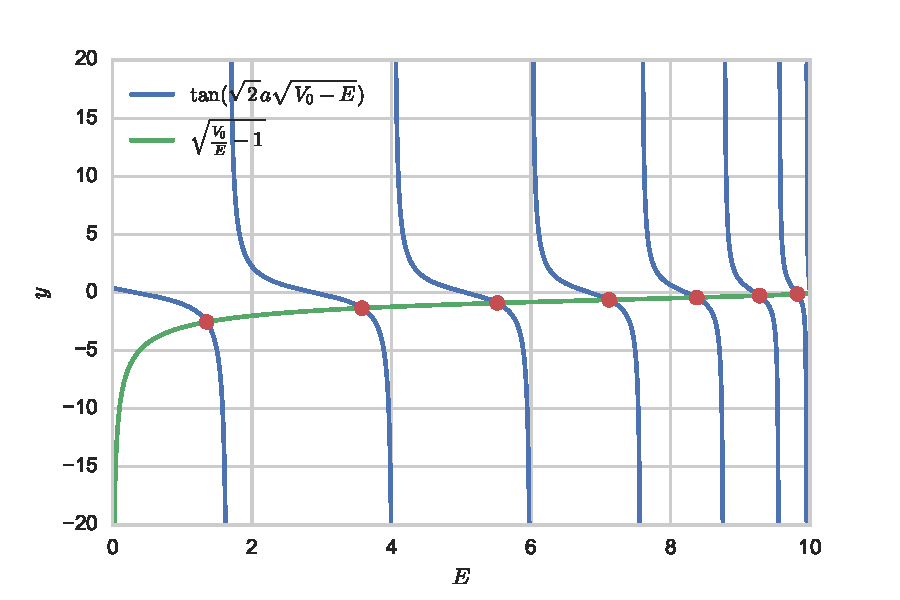
\includegraphics[width=1.0\linewidth]{tan-sqrt.pdf}
  \caption{$\tg \bigg(2V_0a\sqrt{1-\frac{|E|}{V_0}}\bigg)=-\sqrt{\frac{|E|}{V_0}-1}$}
  \label{fig1:tan-sqrt}
\end{subfigure}%
\begin{subfigure}{.5\textwidth}
  \centering
  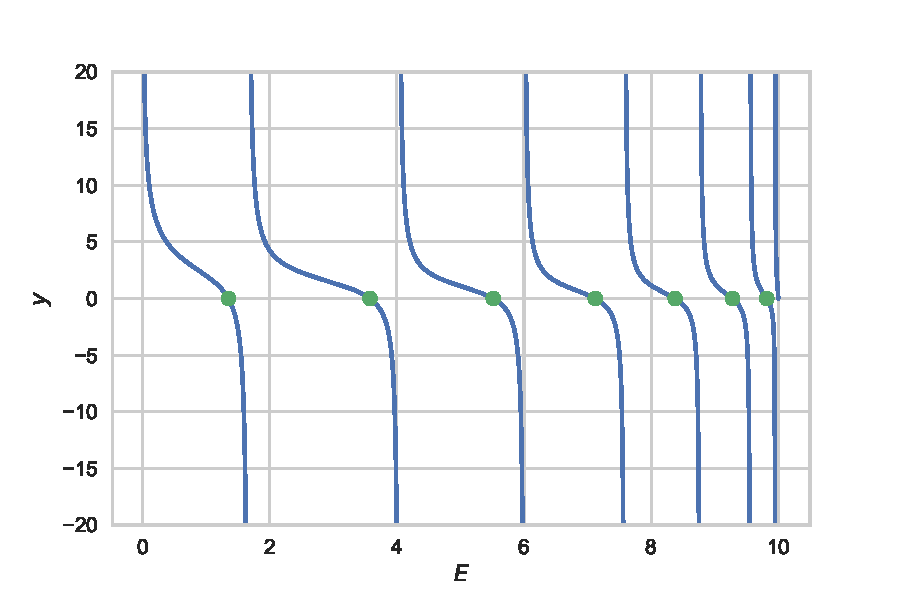
\includegraphics[width=1.0\linewidth]{finite_well.pdf}
  \caption{$\tg \bigg(2V_0a\sqrt{1-\frac{|E|}{V_0}}\bigg)+\sqrt{\frac{|E|}{V_0}-1}=0$}
  \label{fig:finite_well_sol}
\end{subfigure}
\caption{Graphic Illustration of Solutions}
\label{fig:fin_well}
\end{figure}

Some results for energy are following: 
$$0.18021667  ~~0.76501696 ~~ 1.34133445 ~~ 1.90238987~~  2.44644499 ~~ 2.97272142,$$
these values are marked by points on the graphics.

























%$$\lambda \sin^2 {\theta}+\frac{\sin{\theta}}{\theta}\frac{\d}{\d \theta}$$

\bibliography{electron}
\bibliographystyle{plain}
\end{document}
	
	